\documentclass{article}

\usepackage[landscape]{geometry}
\usepackage{url}
\usepackage{amsmath}
\usepackage{amssymb}
\usepackage{esint}
\usepackage{amsfonts}
\usepackage{tikz}
\usepackage{colortbl}
\usepackage{xcolor}
\usepackage{mathtools}
\usepackage{multicol}
\usepackage{pgfplots}
\usepackage{enumitem}

\makeatletter

\newcommand*\bigcdot{\mathpalette\bigcdot@{.5}}
\newcommand*\bigcdot@[2]{\mathbin{\vcenter{\hbox{\scalebox{#2}{$\m@th#1\bullet$}}}}}
\makeatother

\usepackage[english]{babel}
\usepackage[utf8]{inputenc}

\advance\topmargin-.8in
\advance\textheight3in
\advance\textwidth3in
\advance\oddsidemargin-1.5in
\advance\evensidemargin-1.5in
\parindent0pt
\parskip2pt
\newcommand{\hr}{\centerline{\rule{3.5in}{1pt}}}

\tikzstyle{mybox} = [draw=black, fill=white, very thick,
    rectangle, inner sep=10pt, inner ysep=10pt]
\tikzstyle{fancytitle} =[fill=black, text=white, font=\bfseries]

\newenvironment{note}[1]{
    \def\noteArg{#1}
    \begin{tikzpicture}
        \node [mybox] (box)\bgroup%
            \begin{minipage}{0.3\textwidth}}
            {\end{minipage}
        \egroup;

        \node[fancytitle, right=10pt] at (box.north west) {\noteArg};
    \end{tikzpicture}
}

\begin{document}

\definecolor{zzttqq}{rgb}{0.6,0.2,0}
\definecolor{qqqqff}{rgb}{0,0,1}
\definecolor{cqcqcq}{rgb}{0.7529411764705882,0.7529411764705882,0.7529411764705882}

\begin{center}{\huge{\textbf{Coordinate Geometry: The Line}}}\\
\end{center}
\begin{multicols*}{3}

\begin{note}{Distance Between Points}
\small
Distance between $A(x_1, y_1)$ and $B(x_2, y_2)$:
$$
\pm \frac{-b + \sqrt{b^2 - 4ac}}{2a}
$$
\end{note}

\begin{note}{Midpoints of a Line Segment}
\small
Midpoint of line segment between $A(x_1, y_1)$ and $B(x_2, y_2)$:
$$
(\frac{x_1 + x_2}{2}, \frac{y_1 + y_2}{2})
$$
\end{note}

\begin{note}{Slope of a Line}
\small
Choose two points for $(x_1, y_1)$ and $(x_2, y_2)$. The slope is:
$$
m = \frac{\Delta y}{\Delta x} = \frac{\text{rise}}{\text{run}} = \frac{y_2 - y_1}{x_2 - x_1}
$$
\end{note}

\begin{note}{Parallel and Perpendicular Slopes}
\small
1. Two lines are $\parallel$ (parallel) if their slopes are equal.\\
2. Two lines are $\perp$ (perpendicular) if their slopes are negative reciprocals ($m_2 = -1 / m_1$).
\end{note}

\begin{note}{Area of a Triangle}
\small
The area of a triangle with vertices $(0,0)$, $(x_1, y_1)$, and $(x_2, y_2)$ is:

$$
\text{Area} = \frac{1}{2} \lvert x_1 y_2 - x_2 y_1\lvert
$$

\begin{center}
	
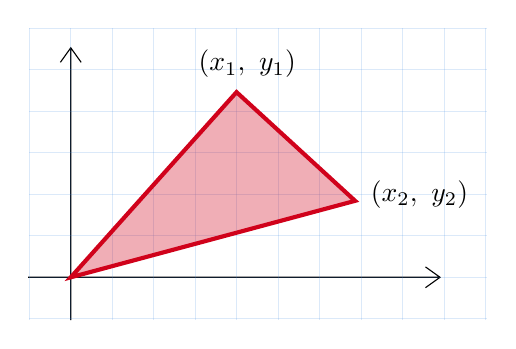
\begin{tikzpicture}[x=0.75pt,y=0.75pt,yscale=-1,xscale=1]
%uncomment if require: \path (0,300); %set diagram left start at 0, and has height of 300

%Shape: Axis 2D [id:dp046860471178072016] 
\draw  (60.5,203.77) -- (258.9,203.77)(81,93.2) -- (81,224.43) (251.9,198.77) -- (258.9,203.77) -- (251.9,208.77) (76,100.2) -- (81,93.2) -- (86,100.2)  ;
%Shape: Grid [id:dp33810988130484365] 
\draw  [draw opacity=0] (61,83.77) -- (281.5,83.77) -- (281.5,224.43) -- (61,224.43) -- cycle ; \draw  [color={rgb, 255:red, 74; green, 144; blue, 226 }  ,draw opacity=0.2 ] (61,83.77) -- (61,224.43)(81,83.77) -- (81,224.43)(101,83.77) -- (101,224.43)(121,83.77) -- (121,224.43)(141,83.77) -- (141,224.43)(161,83.77) -- (161,224.43)(181,83.77) -- (181,224.43)(201,83.77) -- (201,224.43)(221,83.77) -- (221,224.43)(241,83.77) -- (241,224.43)(261,83.77) -- (261,224.43)(281,83.77) -- (281,224.43) ; \draw  [color={rgb, 255:red, 74; green, 144; blue, 226 }  ,draw opacity=0.2 ] (61,83.77) -- (281.5,83.77)(61,103.77) -- (281.5,103.77)(61,123.77) -- (281.5,123.77)(61,143.77) -- (281.5,143.77)(61,163.77) -- (281.5,163.77)(61,183.77) -- (281.5,183.77)(61,203.77) -- (281.5,203.77)(61,223.77) -- (281.5,223.77) ; \draw  [color={rgb, 255:red, 74; green, 144; blue, 226 }  ,draw opacity=0.2 ]  ;
%Shape: Triangle [id:dp2022772656497721] 
\draw  [color={rgb, 255:red, 208; green, 2; blue, 27 }  ,draw opacity=1 ][fill={rgb, 255:red, 208; green, 2; blue, 27 }  ,fill opacity=0.32 ][line width=1.5]  (160.87,114.56) -- (217.98,166.93) -- (81,203.77) -- cycle ;

% Text Node
\draw (166,101) node   {$( x_{1} ,\ y_{1})$};
% Text Node
\draw (249,164) node   {$( x_{2} ,\ y_{2})$};


\end{tikzpicture}
\end{center}

\noindent
You may need to translate the triangle to get one of the vertices to $(0,0)$.
\end{note}

\begin{note}{Dividing a Line Segment by a Given Ratio}
\small
Below, the point $P$ divides the segment in the ratio $a:b$. The coordinates of $P$ are:
$$
P = (\frac{bx_1 + ax_2}{b + a}, \frac{by_1 + ay_2}{b + a})
$$

\begin{center}     
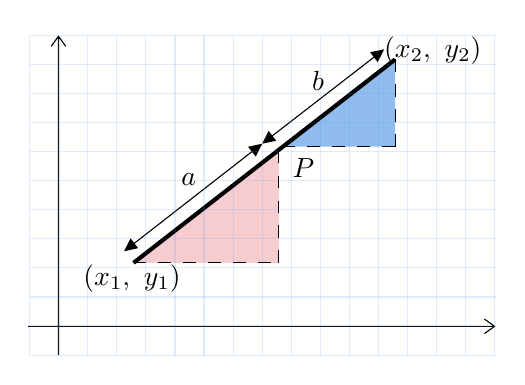
\begin{tikzpicture}[x=0.75pt,y=0.75pt,yscale=-0.7,xscale=0.7]
%uncomment if require: \path (0,300); %set diagram left start at 0, and has height of 300

%Shape: Right Triangle [id:dp6793096363229405] 
\draw  [draw opacity=0][fill={rgb, 255:red, 74; green, 144; blue, 226 }  ,fill opacity=0.61 ] (301,34) -- (223.5,93) -- (301,93) -- cycle ;
%Shape: Right Triangle [id:dp26697740704976447] 
\draw  [draw opacity=0][fill={rgb, 255:red, 208; green, 2; blue, 27 }  ,fill opacity=0.2 ] (221,93.89) -- (121,173) -- (221,173) -- cycle ;
%Shape: Axis 2D [id:dp046860471178072016] 
\draw  (48.5,216.67) -- (369.5,216.67)(69.33,17) -- (69.33,236.5) (362.5,211.67) -- (369.5,216.67) -- (362.5,221.67) (64.33,24) -- (69.33,17) -- (74.33,24)  ;
%Straight Lines [id:da00249800821720636] 
\draw [line width=1.5]    (121,173) -- (301,33) ;


%Straight Lines [id:da4880899923255422] 
\draw  [dash pattern={on 4.5pt off 4.5pt}]  (121,173) -- (221,173) ;


%Straight Lines [id:da3674127553003306] 
\draw  [dash pattern={on 4.5pt off 4.5pt}]  (221,173) -- (221,93) ;


%Straight Lines [id:da9659600918979918] 
\draw  [dash pattern={on 4.5pt off 4.5pt}]  (301,93) -- (301,33) ;


%Straight Lines [id:da3130351016223586] 
\draw  [dash pattern={on 4.5pt off 4.5pt}]  (223.5,93) -- (301,93) ;


%Straight Lines [id:da7491469628550902] 
\draw    (116.08,163.77) -- (207.92,92.23) ;
\draw [shift={(209.5,91)}, rotate = 502.08] [fill={rgb, 255:red, 0; green, 0; blue, 0 }  ][line width=0.75]  [draw opacity=0] (8.93,-4.29) -- (0,0) -- (8.93,4.29) -- cycle    ;
\draw [shift={(114.5,165)}, rotate = 322.08] [fill={rgb, 255:red, 0; green, 0; blue, 0 }  ][line width=0.75]  [draw opacity=0] (8.93,-4.29) -- (0,0) -- (8.93,4.29) -- cycle    ;
%Straight Lines [id:da5539504217371967] 
\draw    (211.08,89.78) -- (291.92,27.22) ;
\draw [shift={(293.5,26)}, rotate = 502.27] [fill={rgb, 255:red, 0; green, 0; blue, 0 }  ][line width=0.75]  [draw opacity=0] (8.93,-4.29) -- (0,0) -- (8.93,4.29) -- cycle    ;
\draw [shift={(209.5,91)}, rotate = 322.27] [fill={rgb, 255:red, 0; green, 0; blue, 0 }  ][line width=0.75]  [draw opacity=0] (8.93,-4.29) -- (0,0) -- (8.93,4.29) -- cycle    ;
%Shape: Grid [id:dp6726746600532687] 
\draw  [draw opacity=0] (49.5,16.5) -- (370.5,16.5) -- (370.5,237) -- (49.5,237) -- cycle ; \draw  [color={rgb, 255:red, 74; green, 144; blue, 226 }  ,draw opacity=0.17 ] (49.5,16.5) -- (49.5,237)(69.5,16.5) -- (69.5,237)(89.5,16.5) -- (89.5,237)(109.5,16.5) -- (109.5,237)(129.5,16.5) -- (129.5,237)(149.5,16.5) -- (149.5,237)(169.5,16.5) -- (169.5,237)(189.5,16.5) -- (189.5,237)(209.5,16.5) -- (209.5,237)(229.5,16.5) -- (229.5,237)(249.5,16.5) -- (249.5,237)(269.5,16.5) -- (269.5,237)(289.5,16.5) -- (289.5,237)(309.5,16.5) -- (309.5,237)(329.5,16.5) -- (329.5,237)(349.5,16.5) -- (349.5,237)(369.5,16.5) -- (369.5,237) ; \draw  [color={rgb, 255:red, 74; green, 144; blue, 226 }  ,draw opacity=0.17 ] (49.5,16.5) -- (370.5,16.5)(49.5,36.5) -- (370.5,36.5)(49.5,56.5) -- (370.5,56.5)(49.5,76.5) -- (370.5,76.5)(49.5,96.5) -- (370.5,96.5)(49.5,116.5) -- (370.5,116.5)(49.5,136.5) -- (370.5,136.5)(49.5,156.5) -- (370.5,156.5)(49.5,176.5) -- (370.5,176.5)(49.5,196.5) -- (370.5,196.5)(49.5,216.5) -- (370.5,216.5)(49.5,236.5) -- (370.5,236.5) ; \draw  [color={rgb, 255:red, 74; green, 144; blue, 226 }  ,draw opacity=0.17 ]  ;

% Text Node
\draw (159,116) node   {$a$};
% Text Node
\draw (248,48) node   {$b$};
% Text Node
\draw (120,184) node   {$( x_{1} ,\ y_{1})$};
% Text Node
\draw (327,27) node   {$( x_{2} ,\ y_{2})$};
% Text Node
\draw (238,108) node   {$P$};


\end{tikzpicture}
\end{center}
\end{note}


\begin{note}{Triangle Concurrency: Centroid}
\small
Intersection of the medians. Point given by
$$
P = (\frac{x_1 + x_2 + x_3}{3}, \frac{y_1 + y_2 + y_3}{3})
$$

\begin{center}     

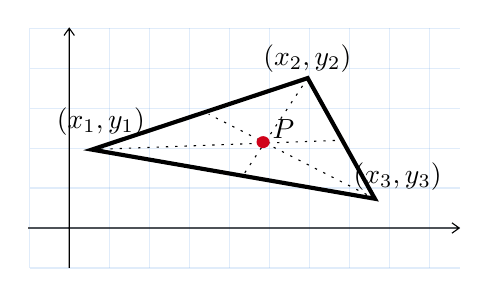
\begin{tikzpicture}[x=0.75pt,y=0.75pt,yscale=-0.5,xscale=0.5]
%uncomment if require: \path (0,300); %set diagram left start at 0, and has height of 300

%Shape: Grid [id:dp6726746600532687] 
\draw  [draw opacity=0] (25.61,51.98) -- (440.5,51.98) -- (440.5,283) -- (25.61,283) -- cycle ; \draw  [color={rgb, 255:red, 74; green, 144; blue, 226 }  ,draw opacity=0.17 ] (25.61,51.98) -- (25.61,283)(64.11,51.98) -- (64.11,283)(102.61,51.98) -- (102.61,283)(141.11,51.98) -- (141.11,283)(179.61,51.98) -- (179.61,283)(218.11,51.98) -- (218.11,283)(256.61,51.98) -- (256.61,283)(295.12,51.98) -- (295.12,283)(333.62,51.98) -- (333.62,283)(372.12,51.98) -- (372.12,283)(410.62,51.98) -- (410.62,283) ; \draw  [color={rgb, 255:red, 74; green, 144; blue, 226 }  ,draw opacity=0.17 ] (25.61,51.98) -- (440.5,51.98)(25.61,90.48) -- (440.5,90.48)(25.61,128.98) -- (440.5,128.98)(25.61,167.48) -- (440.5,167.48)(25.61,205.98) -- (440.5,205.98)(25.61,244.48) -- (440.5,244.48)(25.61,282.98) -- (440.5,282.98) ; \draw  [color={rgb, 255:red, 74; green, 144; blue, 226 }  ,draw opacity=0.17 ]  ;
%Shape: Axis 2D [id:dp0800302445778831] 
\draw  (24,244.5) -- (439.29,244.5)(63.49,51.98) -- (63.49,282.98) (432.29,239.5) -- (439.29,244.5) -- (432.29,249.5) (58.49,58.98) -- (63.49,51.98) -- (68.49,58.98)  ;
%Shape: Triangle [id:dp29121420214390215] 
\draw  [line width=1.5]  (293.3,100.05) -- (358.03,216.29) -- (85.26,168.93) -- cycle ;
%Straight Lines [id:da4728550289451101] 
\draw  [dash pattern={on 0.84pt off 2.51pt}]  (293.29,100.07) -- (231.78,192.55) ;


%Straight Lines [id:da5866394717552575] 
\draw  [dash pattern={on 0.84pt off 2.51pt}]  (85.26,168.91) -- (327.68,159.82) ;


%Straight Lines [id:da8957549944298021] 
\draw  [dash pattern={on 0.84pt off 2.51pt}]  (358.03,216.29) -- (197.93,134.79) ;


%Shape: Ellipse [id:dp868924086338054] 
\draw  [draw opacity=0][fill={rgb, 255:red, 208; green, 2; blue, 27 }  ,fill opacity=1 ] (244,161.73) .. controls (244,158.55) and (246.83,155.97) .. (250.31,155.97) .. controls (253.79,155.97) and (256.61,158.55) .. (256.61,161.73) .. controls (256.61,164.9) and (253.79,167.48) .. (250.31,167.48) .. controls (246.83,167.48) and (244,164.9) .. (244,161.73) -- cycle ;

% Text Node
\draw (270,149) node   {$P$};
% Text Node
\draw (94,142) node   {$( x_{1} ,y_{1})$};
% Text Node
\draw (293,81) node   {$( x_{2} ,y_{2})$};
% Text Node
\draw (380,195) node   {$( x_{3} ,y_{3})$};


\end{tikzpicture}

\end{center}
\end{note}

\begin{note}{Triangle Concurrency: Circumcentre}
\small
Intersection of the perpendicular bisectors, and center of the circumcircle.
\begin{center}     
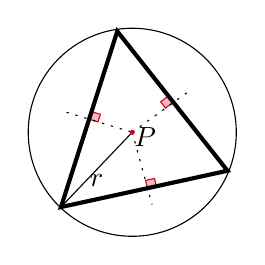
\begin{tikzpicture}[x=0.75pt,y=0.75pt,yscale=-0.5,xscale=0.5]
%uncomment if require: \path (0,300); %set diagram left start at 0, and has height of 300

%Straight Lines [id:da6714428869151924] 
\draw    (149.55,223.32) -- (218.25,151.25) ;


%Shape: Rectangle [id:dp03924467384504826] 
\draw  [color={rgb, 255:red, 208; green, 2; blue, 27 }  ,draw opacity=1 ][fill={rgb, 255:red, 208; green, 2; blue, 27 }  ,fill opacity=0.28 ] (231.07,197.65) -- (239.7,195.7) -- (241.38,203.13) -- (232.75,205.09) -- cycle ;
%Shape: Rectangle [id:dp6487935341462473] 
\draw  [color={rgb, 255:red, 208; green, 2; blue, 27 }  ,draw opacity=1 ][fill={rgb, 255:red, 208; green, 2; blue, 27 }  ,fill opacity=0.28 ] (245.64,121.93) -- (252.6,116.46) -- (257.31,122.46) -- (250.35,127.93) -- cycle ;
%Shape: Rectangle [id:dp8771618985154196] 
\draw  [color={rgb, 255:red, 208; green, 2; blue, 27 }  ,draw opacity=1 ][fill={rgb, 255:red, 208; green, 2; blue, 27 }  ,fill opacity=0.28 ] (179.05,131.37) -- (187.5,134) -- (185.24,141.28) -- (176.79,138.66) -- cycle ;
%Shape: Circle [id:dp006062218319284107] 
\draw   (118,151.25) .. controls (118,95.88) and (162.88,51) .. (218.25,51) .. controls (273.62,51) and (318.5,95.88) .. (318.5,151.25) .. controls (318.5,206.62) and (273.62,251.5) .. (218.25,251.5) .. controls (162.88,251.5) and (118,206.62) .. (118,151.25) -- cycle ;
%Shape: Triangle [id:dp8510805191799975] 
\draw  [line width=1.5]  (203.82,53.96) -- (310,188.33) -- (149.55,223.32) -- cycle ;
%Straight Lines [id:da6999380610647019] 
\draw  [dash pattern={on 0.84pt off 2.51pt}]  (154.88,132) -- (218.25,151.25) ;


%Straight Lines [id:da5161798596139192] 
\draw  [dash pattern={on 0.84pt off 2.51pt}]  (218.25,151.25) -- (237.33,221) ;


%Straight Lines [id:da005399746280609574] 
\draw  [dash pattern={on 0.84pt off 2.51pt}]  (218.25,151.25) -- (272,112.33) ;


%Shape: Circle [id:dp8548778581188706] 
\draw  [draw opacity=0][fill={rgb, 255:red, 208; green, 2; blue, 27 }  ,fill opacity=1 ] (215.88,151.25) .. controls (215.88,149.94) and (216.94,148.88) .. (218.25,148.88) .. controls (219.56,148.88) and (220.62,149.94) .. (220.62,151.25) .. controls (220.62,152.56) and (219.56,153.62) .. (218.25,153.62) .. controls (216.94,153.62) and (215.88,152.56) .. (215.88,151.25) -- cycle ;

% Text Node
\draw (230.67,156) node   {$P$};
% Text Node
\draw (184,197.67) node   {$r$};


\end{tikzpicture}
\end{center}
\end{note}

\begin{note}{Triangle Concurrency: Orthocentre}
\small
The intersection of the perpendiculars from the vertices to the opposite sides.
\begin{center}     
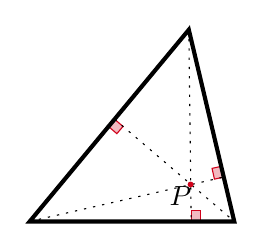
\begin{tikzpicture}[x=0.75pt,y=0.75pt,yscale=-0.6,xscale=0.6]
%uncomment if require: \path (0,300); %set diagram left start at 0, and has height of 300

%Shape: Rectangle [id:dp06651470372425916] 
\draw  [color={rgb, 255:red, 208; green, 2; blue, 27 }  ,draw opacity=1 ][fill={rgb, 255:red, 208; green, 2; blue, 27 }  ,fill opacity=0.28 ] (194.77,126.23) -- (201.49,131.99) -- (196.53,137.78) -- (189.81,132.02) -- cycle ;
%Shape: Rectangle [id:dp1415385076092982] 
\draw  [color={rgb, 255:red, 208; green, 2; blue, 27 }  ,draw opacity=1 ][fill={rgb, 255:red, 208; green, 2; blue, 27 }  ,fill opacity=0.28 ] (280.42,164) -- (282.35,172.64) -- (274.91,174.3) -- (272.98,165.67) -- cycle ;
%Shape: Rectangle [id:dp8771618985154196] 
\draw  [color={rgb, 255:red, 208; green, 2; blue, 27 }  ,draw opacity=1 ][fill={rgb, 255:red, 208; green, 2; blue, 27 }  ,fill opacity=0.28 ] (263.88,199.81) -- (263.88,208.66) -- (256.26,208.66) -- (256.26,199.81) -- cycle ;
%Shape: Triangle [id:dp8510805191799975] 
\draw  [line width=1.5]  (254.33,54.35) -- (290.82,208.26) -- (126.6,208.26) -- cycle ;
%Straight Lines [id:da6999380610647019] 
\draw  [dash pattern={on 0.84pt off 2.51pt}]  (126.6,208.26) -- (282.33,172.67) ;


%Straight Lines [id:da5161798596139192] 
\draw  [dash pattern={on 0.84pt off 2.51pt}]  (254.33,54.35) -- (256.26,209.66) ;


%Straight Lines [id:da0920527477815749] 
\draw  [dash pattern={on 0.84pt off 2.51pt}]  (194.77,126.23) -- (290.82,208.26) ;


%Shape: Circle [id:dp8548778581188706] 
\draw  [draw opacity=0][fill={rgb, 255:red, 208; green, 2; blue, 27 }  ,fill opacity=1 ] (253.38,178.58) .. controls (253.38,177.28) and (254.44,176.22) .. (255.75,176.22) .. controls (257.06,176.22) and (258.12,177.28) .. (258.12,178.58) .. controls (258.12,179.89) and (257.06,180.95) .. (255.75,180.95) .. controls (254.44,180.95) and (253.38,179.89) .. (253.38,178.58) -- cycle ;

% Text Node
\draw (247.53,187.93) node   {$P$};


\end{tikzpicture}
\end{center}
\end{note}


\begin{note}{Perpendicular Distance: Point to a Line}
\small
The perpendicular distance $d$ from a point $(x_1, y_1)$ to a line $ax + by + c=0$ is:
$$
d = \frac{\lvert ax_1 + by_2 + c\lvert}{\sqrt{a^2 + b^2}}
$$
\begin{center}    


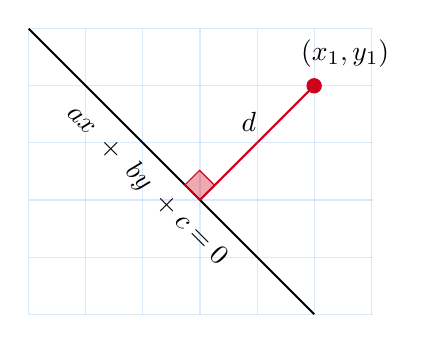
\begin{tikzpicture}[x=0.75pt,y=0.75pt,yscale=-0.8,xscale=0.8]
%uncomment if require: \path (0,300); %set diagram left start at 0, and has height of 300

%Straight Lines [id:da4556507051008317] 
\draw [color={rgb, 255:red, 208; green, 2; blue, 27 }  ,draw opacity=1 ][line width=0.75]    (214.33,130.37) -- (283.09,61.61) ;


%Shape: Grid [id:dp8283162598083013] 
\draw  [draw opacity=0] (111.19,27.23) -- (318.5,27.23) -- (318.5,199.82) -- (111.19,199.82) -- cycle ; \draw  [color={rgb, 255:red, 74; green, 144; blue, 226 }  ,draw opacity=0.2 ] (111.19,27.23) -- (111.19,199.82)(145.57,27.23) -- (145.57,199.82)(179.95,27.23) -- (179.95,199.82)(214.33,27.23) -- (214.33,199.82)(248.71,27.23) -- (248.71,199.82)(283.09,27.23) -- (283.09,199.82)(317.47,27.23) -- (317.47,199.82) ; \draw  [color={rgb, 255:red, 74; green, 144; blue, 226 }  ,draw opacity=0.2 ] (111.19,27.23) -- (318.5,27.23)(111.19,61.61) -- (318.5,61.61)(111.19,95.99) -- (318.5,95.99)(111.19,130.37) -- (318.5,130.37)(111.19,164.75) -- (318.5,164.75)(111.19,199.13) -- (318.5,199.13) ; \draw  [color={rgb, 255:red, 74; green, 144; blue, 226 }  ,draw opacity=0.2 ]  ;
%Straight Lines [id:da9663943139290453] 
\draw [line width=0.75]    (111.19,27.23) -- (283.09,199.13) ;


%Shape: Ellipse [id:dp268126665598059] 
\draw  [draw opacity=0][fill={rgb, 255:red, 208; green, 2; blue, 27 }  ,fill opacity=1 ] (278.45,61.61) .. controls (278.45,59.04) and (280.52,56.96) .. (283.09,56.96) .. controls (285.65,56.96) and (287.73,59.04) .. (287.73,61.61) .. controls (287.73,64.17) and (285.65,66.25) .. (283.09,66.25) .. controls (280.52,66.25) and (278.45,64.17) .. (278.45,61.61) -- cycle ;
%Shape: Rectangle [id:dp6643318066156415] 
\draw  [color={rgb, 255:red, 208; green, 2; blue, 27 }  ,draw opacity=1 ][fill={rgb, 255:red, 208; green, 2; blue, 27 }  ,fill opacity=0.34 ] (214.11,112.53) -- (223.14,121.56) -- (214.33,130.37) -- (205.3,121.34) -- cycle ;

% Text Node
\draw (301.77,42.26) node   {$( x_{1} ,y_{1})$};
% Text Node
\draw (182.35,121.65) node [rotate=-45]  {$ax\ +\ by\ +c=0$};
% Text Node
\draw (243.77,83.26) node   {$d$};


\end{tikzpicture}

\end{center}
\end{note}


\begin{note}{Angle Between Two Lines}
\small
The angle $\theta$ between two lines with slopes $m_1$ and $m_2$ as shown is given by:
$$
\tan \theta = \pm \frac{m_1 - m_2}{1 + m_1 m_2}
$$
\begin{center}    

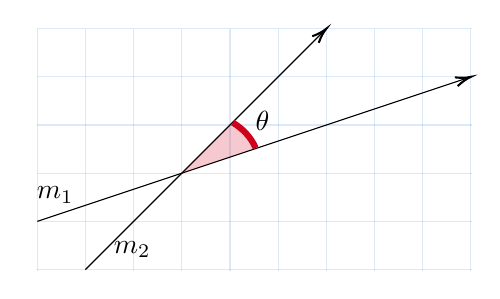
\begin{tikzpicture}[x=0.75pt,y=0.75pt,yscale=-0.675,xscale=0.675]
%uncomment if require: \path (0,300); %set diagram left start at 0, and has height of 300

%Shape: Grid [id:dp8283162598083013] 
\draw  [draw opacity=0] (155.19,53.23) -- (465.14,53.23) -- (465.14,225.82) -- (155.19,225.82) -- cycle ; \draw  [color={rgb, 255:red, 74; green, 144; blue, 226 }  ,draw opacity=0.2 ] (155.19,53.23) -- (155.19,225.82)(189.57,53.23) -- (189.57,225.82)(223.95,53.23) -- (223.95,225.82)(258.33,53.23) -- (258.33,225.82)(292.71,53.23) -- (292.71,225.82)(327.09,53.23) -- (327.09,225.82)(361.47,53.23) -- (361.47,225.82)(395.85,53.23) -- (395.85,225.82)(430.23,53.23) -- (430.23,225.82)(464.61,53.23) -- (464.61,225.82) ; \draw  [color={rgb, 255:red, 74; green, 144; blue, 226 }  ,draw opacity=0.2 ] (155.19,53.23) -- (465.14,53.23)(155.19,87.61) -- (465.14,87.61)(155.19,121.99) -- (465.14,121.99)(155.19,156.37) -- (465.14,156.37)(155.19,190.75) -- (465.14,190.75)(155.19,225.13) -- (465.14,225.13) ; \draw  [color={rgb, 255:red, 74; green, 144; blue, 226 }  ,draw opacity=0.2 ]  ;
%Straight Lines [id:da5993219790582195] 
\draw    (155.19,190.75) -- (462.71,88.24) ;
\draw [shift={(464.61,87.61)}, rotate = 521.5699999999999] [color={rgb, 255:red, 0; green, 0; blue, 0 }  ][line width=0.75]    (10.93,-3.29) .. controls (6.95,-1.4) and (3.31,-0.3) .. (0,0) .. controls (3.31,0.3) and (6.95,1.4) .. (10.93,3.29)   ;

%Straight Lines [id:da891181685289479] 
\draw    (189.57,225.13) -- (360.05,54.64) ;
\draw [shift={(361.47,53.23)}, rotate = 495] [color={rgb, 255:red, 0; green, 0; blue, 0 }  ][line width=0.75]    (10.93,-3.29) .. controls (6.95,-1.4) and (3.31,-0.3) .. (0,0) .. controls (3.31,0.3) and (6.95,1.4) .. (10.93,3.29)   ;

%Shape: Arc [id:dp5545044854551309] 
\draw  [draw opacity=0][fill={rgb, 255:red, 208; green, 2; blue, 27 }  ,fill opacity=0.21 ][line width=2.25]  (294.75,120.27) .. controls (302.11,124.76) and (307.82,130.92) .. (311,138.34) -- (258.33,156.37) -- cycle ; \draw  [color={rgb, 255:red, 208; green, 2; blue, 27 }  ,draw opacity=1 ][line width=2.25]  (294.75,120.27) .. controls (302.11,124.76) and (307.82,130.92) .. (311,138.34) ;

% Text Node
\draw (316,119) node   {$\theta $};
% Text Node
\draw (168,172) node   {$m_{1}$};
% Text Node
\draw (223,211) node   {$m_{2}$};


\end{tikzpicture}\end{center}
\end{note}
    
\end{multicols*}
\end{document}